\subsection{Propulsion (PRP)}

The propulsion subsystem is responsible for changing the spacecraft's orbit. In the first phase of the cubesat lifetime, propulsion is necessary for proper satellite positioning as well as minor orbit corrections and collision avoidance during the remainder of its lifetime. To position the satellites, their time-position must be  adjusted. The aim is to create a constellation of satellites to provide complete communications coverage over the Earth's surface. The proposed constellation shall be composed of 8 polar orbiting families of satellites. Each family shall be comprised of 9 cubesats.

Changing the time-position of one satellite along the orbit is known as \textbf{orbit phasing}. As shown in Figure \ref{fig:orbit_phasing} the satellite can be given an increase in velocity to lower the orbital altitude, thus decreasing the orbital period. When the satellite completes the phasing orbit, another velocity change is required to return the satellite to the desired orbit.

\begin{figure}[h!]
	\centering
	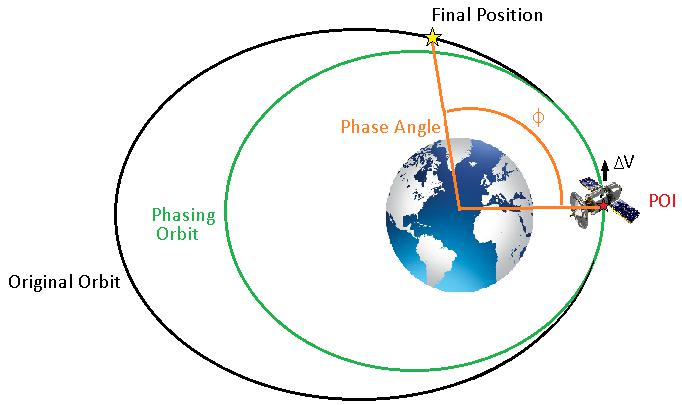
\includegraphics[scale=0.5]{img/Orbit_Phase.jpg}
	\caption{Orbit Phasing}
	\label{fig:orbit_phasing}
\end{figure}

\subsubsection{Impulsive Maneuvers} \label{Impulsive}

There are a number of methods of achieving the desired orbits for this constellation.
\begin{enumerate}
	\item Differing $\Delta V$
	In this scenario, nine satellites are launched into polar orbit at an altitude of 625km, the desired orbit. Each satellite then does one phasing orbit, using differing $\Delta V$ and returns to it's polar orbit. This method is the fastest but requires different amounts of propellant for each satellite.
	\item Differing number of phasing orbits.
	Here, the satellites are launched to the same orbit as in the previous case. However, each satellite, except one, experiences the same $\Delta V$ but they complete a different number of phasing orbits before returning to their original orbit. If we number the satellites as n=1:9, then satellite n will complete n-1 phasing orbits. This method is slower than the first method but it involves significantly less propellant as n increases.
	\item Launch to phasing orbit
	The third method is to launch all nine satellites to the 'phasing orbit'. As with method 2, the satellites would complete n-1 phasing orbits before using a velocity kick to reach the desired orbit. The benefit of this method is that eight of the satellites would only need one velocity change, rather than two, however, satellite 1 in the orbital family would need one extra velocity kick. Clearly, method 3 uses the least amount of propellant of all three methods, while also having the benefit of standardising the satellites' propulsion systems as each one would require an equal amount of propellant.
\end{enumerate}

For the following analysis, method three will be used.

\paragraph{Required $\Delta V$}
For an orbit of nine satellites, $\phi = 40^{\circ}$. To calculate the required $\Delta V$ the following equations can be used, where subscript 1 refers to the original orbit and subscript 2 refers to the final orbit.

\begin{equation}
	E=2tan^{-1}\bigg(\sqrt{\frac{1-e_1}{1+e_1}tan\frac{\phi}{2}} \bigg)
	\label{MMeq1}
\end{equation}

\begin{equation}
	t=\frac{T_1}{2\pi}(E - e_1 sinE)
	\label{MMeq2}
\end{equation}

The required time period of the final orbit is then given by using equation \ref{MMeq3}.

\begin{equation}
	T_2 = T_1 -t
	\label{MMeq3}
\end{equation}

The final orbit semimajor axis can then be determined by using equation \ref{MMeq4}.

\begin{equation}
	a_2 = \bigg(\frac{\sqrt{\mu}T_2}{2\pi}\bigg)^{\frac{2}{3}}
	\label{MMeq4}
\end{equation}

The angular momentum of the orbit can then be calculated by using equation \ref{MMeq5}.

\begin{equation}
	h_2 = \sqrt{2\mu}\sqrt{\frac{r_ar_p}{r_a+r_p}}
	\label{MMeq5}
\end{equation}

Finally, equation \ref{MMeq6} can be used to calculate the change in velocity, $\Delta V$ at the Point of Impulse.

\begin{equation}
	\Delta V = v_2 - v_1 = \frac{h_2}{r}-\frac{h_1}{r}
	\label{MMeq6}
\end{equation}

The result of these calculations shows that a $\Delta V$ of $350 m/s$ is needed to transfer from the phasing orbit to the circular constellation orbit.

\paragraph{Propellant Mass Fraction}
With the required $\Delta V$ known, the Tsiolkovsky rocket equation (equation \ref{MMeq7}) can be derived to estimate the required mass fraction of propellant for various propulsion systems (equation \ref{MMeq8}). To do this, the effective exhaust velocity of the thruster must be known.

\begin{equation}
	\Delta V = v_e ln \frac{m_0}{m_f}
	\label{MMeq7}
\end{equation}

\begin{equation}
	\frac{m_p}{m_0} = 1-exp\bigg(-\frac{\Delta V}{v_e}\bigg)
	\label{MMeq8}
\end{equation}

As $v_e = g_0 I_{sp}$ we can approximate the mass fractions of propellant needed for a variety of thrusters of given $I_{sp}$, by Tummala and Dutta in \cite{Tummala}. From the previous equations, it is clear that a high $I_{sp}$ is desirable to minimise the mass fraction of the propellant, and thereby the mass of the propulsion system. Here, the propulsion system with the greatest Specific Impulse of each propellant type, except solar sails, is examined.

\begin{table}[h!]
	\centering
	\begin{tabular}{c c c c c c }
		\hline
		Propellant & Manufacturer & Engine & $I_{sp}(s)$ & $v_e(m/s)$ & $m_p/m_0$ \\
		\hline
		Cold Gas & GOMSpace & MEMS Cold Gas & 62 & 608.22 & 0.438 \\
		Liquid & Tethers Unlimited & HYDROS & 256 & 2511.36 & 0.130 \\
		Solid & Orbital ATK & STAR 4G & 269.4 & 2642.814 & 0.124 \\
		Resistojet & Busek & AMR & 150 & 1471.5 & 0.212 \\
		Radio Frequency Ion & Busek & BIT-3 & 2500 & 24525 & 0.014 \\
		Hall Effect & Sitael Aerospace & HT 400 & 1750 & 17167.5 & 0.020 \\
		Electrospray & Busek & BET-100 & 1800 & 17658 & 0.019 \\
		Arc Thrusters & Busek & MPACS & 830 & 8142.3 & 0.042 \\
		\hline
	\end{tabular}
	\caption{$I_{sp}$ and $v_e$ for various cubesat propulsion systems with corresponding mass fraction of propellant needed to obtain $\Delta V$ of $350 m/s$}
	\label{MMtab1}
\end{table}

Proceeding with the six engines which require less than 20\% propellant mass, the practical limitations of the engines are laid out in table \ref{MMtab2}.
\\
\begin{table}[h!]
	\centering
	\begin{tabular}{c c c c c }
		\hline
		Propellant & Manufacturer & Engine & Thruster Mass(kg) & Power(W) \\
		\hline
		Liquid & Thethers Unlimited & HYDROS & 1.87 & 25 \\
		Solid & Orbital ATK & STAR 4G & 0.52 & N/A \\
		Radio Frequency Ion & Busek & BIT-3 & 0.2 & 20-70 \\
		Hall Effect & Sitael Aerospace & HT 400 & 0.9 & 250-800 \\
		Electrospray & Busek & BET-100 & 0.329 & 5.5 \\
		Arc Thrusters & Busek & MPACS & 0.5 & 7.5 \\
		\hline
	\end{tabular}
	\caption{$I_{sp}$ and $v_e$ for cubesat propulsion systems with corresponding thruster unit mass and nominal power consumption}
	\label{MMtab2}
\end{table}
\\
The solid propellant engine designed by Orbital ATK provides average thrust of 258N. 258N of thrust could give a 4kg satellite a 350m/s velocity change in 5.4 seconds. This could be considered an impulsive maneuver.

Although the power required for this thruster is not available, the description of the engine given by Orbital ATK states that testing and development of the STAR 4G happened in January 2000. The catalogue blurb also states that the engine was developed as a low-cost, high mass fraction orbit adjust motor for use in deploying constellations of very small satellites (nanosatellites)" \cite{STAR4G}.

The maximum propellant mass in the STAR 4G engine is 980 grams. As stated in table \ref{MMtab1}, the required propellant mass fraction for this engine is 0.124. Presuming a 3-U cubesat (4kg), this means the propellant mass would have to be 496 grams to achieve the desired $\Delta V$ to position this constellation. The total wet mass of the propulsion system is then 1.5kg, with a full tank of propellant. However, solid propellant cannot be extinguished once it is ignited so the mass of propellant carried on board the satellites should be exactly 496 grams, resulting in a total wet mass of 1.016 kg.

\subsubsection{Low Thrust Maneuvers}
\paragraph{Required $\Delta V$}
The analysis for obtaining the required $\Delta V$ is similar for low and high thrust maneuvers because the satellite is in almost the same orbit in both cases, even during thrusting periods \cite{MIT}. Also, the $\Delta V$ is equal to the difference between beginning and ending orbital speeds. In practical terms however, the impulsive maneuver examined in \ref{Impulsive} requires a two-impulse Hohmann transfer between orbits, whereas the low thrust transfer uses continuous thrusting. This section will examine the low thrust orbit transfer as analysed in section \ref{Impulsive}, with one change. The orbit into which the satellites will be launched, initially, will be such that the period is  $1/27^{th}$ greater than the desired orbit period. The result is that after three orbits, the satellite will be phased to the desired position, relative to the satellite it follows. The classical orbital elements of such an orbit are easily obtained. The launch orbit will have a period of 6563.9 seconds which is at an average altitude of 1205.48 km above the surface of the earth.

The required $\Delta V$ can be simply calculated as the difference between the two orbital velocities. It is found to be 294.89 m/s.

The Busek BET-100 engine is appropriate for low trust maneuvers with its low mass, propellant mass fraction and power consumption. Electrospray technology use in cubesats is still relatively new after being introduced by NASA and MIT in 2013. There are still system reliability issues related to the scalable thrust and the lifetime of these engines.

The low thrust maneuver offers no significant advantage over the impulsive maneuver, therefore the STAR 4G engine by Orbital ATK will be installed on the nanosatellites.

\paragraph{Chosen Propulsion System}
The Orbital ATK STAR 4G thruster shall be installed in the nanosatellites to provide an impulsive perigee kick maneuver and position the satellites in the desired orbits. The STAR 4G engine shall have a total wet mass of 1.016kg. The thruster's power consumption is not available although it is presumed to be reasonable, as the thruster is designed for positioning nanosatellites in orbit. The operating temperature range for this engine is between $4^\circ C$ and $32^\circ C$. The spherical thruster is 95mm in diameter and 108 mm in length including the nozzle, which has an expansion ratio of 56.8:1.
